\begin{frame}{What did/will we do on Thursday?}

\begin{itemize}
\itemsep1pt\parskip0pt\parsep0pt
\item
  We did/will do a quick overview of probability as you will have
  encountered it in school
\item
  We will have generated some data using dice and coins.
\item
  We will use those data to explore descriptive statistics
\item
  Measures of central tendency such as \emph{mean} and \emph{median}
\item
  Measures of disperson or variability such as variance and standard
  deviation
\end{itemize}

\end{frame}

\begin{frame}{What is advanced about these statistics?}

\begin{itemize}
\itemsep1pt\parskip0pt\parsep0pt
\item
  Goal is for you to understand the principles, not just the steps.
\item
  Simulation approach:
\item
  If you don't know how something about a statistical test, simulate it!
\item
  Example questions you might ask:

  \begin{itemize}
  \itemsep1pt\parskip0pt\parsep0pt
  \item
    What is the power of this test?
  \item
    What happens if I violate the normality assumption for an ANOVA?
  \item
    What happens if I don't correct for multiple comparisons?
  \end{itemize}
\end{itemize}

\end{frame}

\begin{frame}{How do I run simulations?}

\begin{itemize}
\itemsep1pt\parskip0pt\parsep0pt
\item
  Not very easy in SPSS
\item
  But Excel can help (to some degree..)
\item
  For more detailed simulations, you'll have to use a programming
  language such as R, Python, C++, etc.
\end{itemize}

\end{frame}

\begin{frame}{Introduction}

\begin{itemize}
\itemsep1pt\parskip0pt\parsep0pt
\item
  Let's start nice and easy. I brought some dice to class. This was my
  task:

  \begin{itemize}
  \itemsep1pt\parskip0pt\parsep0pt
  \item
    There are dice in 9 different colours
  \item
    I want you to find out if the orange dice are loaded (i.e.~if they
    have the tendency to end up on certain sides more than on others)
  \end{itemize}
\item
  How should you go about this?
\end{itemize}

\end{frame}

\begin{frame}{Maths basics: Summation}

\begin{itemize}
\itemsep1pt\parskip0pt\parsep0pt
\item
  The summation operator \(\Sigma\):
  \[x_1 + x_2 + x_3 + x_4 + x_5 = \sum\limits_{i=1}^5{x_i}\]
\item
  This means: beginning with \(i=1\) and ending with \(i=5\) sum over
  the variables \(x_i\).

  \begin{itemize}
  \itemsep1pt\parskip0pt\parsep0pt
  \item
    This can save a lot of space if you are summing over lots of
    variables
  \item
    \(i\) is called the \emph{index} over which you are summing, and
    \(1\) and \(5\) are the limits.
  \end{itemize}
\item
  If the limits are clear from the context, you can also write this as
\end{itemize}

\[\sum\limits_{i}{x_i}\]

\end{frame}

\begin{frame}{Maths basics: Summation}

\begin{itemize}
\itemsep1pt\parskip0pt\parsep0pt
\item
  The summation operator \(\Sigma\):
  \[x_1 + x_2 + x_3 + x_4 + x_5 = \sum\limits_{i=1}^5{x_i}\]
\item
  This means: beginning with \(i=1\) and ending with \(i=5\) sum over
  the variables \(x_i\).

  \begin{itemize}
  \itemsep1pt\parskip0pt\parsep0pt
  \item
    This can save a lot of space if you are summing over lots of
    variables
  \item
    \(i\) is called the \emph{index} over which you are summing, and
    \(1\) and \(5\) are the limits.
  \end{itemize}
\item
  If the limits are clear from the context, you can also write this as
\end{itemize}

\[\sum\limits_{i}{x_i}\]

\end{frame}

\begin{frame}{Maths basics: Summation (2)}

\begin{itemize}
\itemsep1pt\parskip0pt\parsep0pt
\item
  You can have multiple multiple indices and sum over them (e.g.~if you
  have multiple people in multiple groups, which is something that
  happens in Psychology \emph{ALL THE TIME}). For example:
\end{itemize}

Group 1 (females): \(x_{11}, x_{12}, x_{13}, x_{14}\)

Group 2 (males): \(x_{21}, x_{22}, x_{23}, x_{24}\)

Sum of all the individuals in all the groups:

\[
\begin{aligned}
\sum\limits_{m=1}^{2}\sum\limits_{x=1}^{4}{x_{mi}} = x_{11}+x_{12}+x_{13}+x_{14} \\
  + x_{21} + x_{22} + x_{23} + x_{24}
\end{aligned}
\]

\end{frame}

\begin{frame}{Maths basics: Multiplication}

\begin{itemize}
\itemsep1pt\parskip0pt\parsep0pt
\item
  The product symbol \(\Pi\):
\item
  Works just like the summation symbol:
  \[x_1 \cdot x_2 \cdot x_3 \cdot x_4 \cdot x_5 = \prod\limits_{i=1}^5{x_i}\]
\item
  This means: beginning with \(i=1\) and ending with \(i=5\) calculate
  the product over the variables \(x_i\).
\end{itemize}

\[
\begin{aligned}
\prod\limits_{m=1}^{2}\prod\limits_{x=1}^{4}{x_{mi}} = x_{11}\cdot x_{12}\cdot x_{13}\cdot x_{14} \\
  \cdot x_{21} \cdot x_{22} \cdot x_{23} \cdot x_{24}
\end{aligned}
\]

\end{frame}

\begin{frame}{Maths basics: Probability}

\begin{itemize}
\itemsep1pt\parskip0pt\parsep0pt
\item
  Basic rules:

  \begin{itemize}
  \itemsep1pt\parskip0pt\parsep0pt
  \item
    All probabilities are between 0 and 1: \(P(A)\in[0,1]\)
  \item
    The complementary probability of an event (i.e.~the probability that
    an event will NOT happen) is 1-the probability of the event:
    \(P(A^c)=1-P(A)\)
  \item
    A probability can be interpreted as the number of outcomes that form
    an event (e.g.~the outcome ``Heads'' when flipping a coin) over the
    total number of outcomes (e.g. ``Heads'' and ``Tails'')
    \[ p(A) = \frac{n_A}{n}\]
  \item
    But note that a probability of .5 (e.g.~for getting ``Heads'' on a
    coin flip) doesn't mean that you will get ``Heads'' on exactly 50\%
    of coin flips.
  \end{itemize}
\end{itemize}

\end{frame}

\begin{frame}{Maths basics: Probability (2)}

\begin{itemize}
\itemsep1pt\parskip0pt\parsep0pt
\item
  Basic rules:

  \begin{itemize}
  \item
    What is the probability that Event A and Event B will happen
    together? \[\begin{aligned}
    P(A\cap B) & = P(A|B)P(B) = P(B|A)P(A)\\
    P(A\cap B) &  = P(A)P(B) \qquad\\&\mbox{if A and B are independent}\\
    \end{aligned}\]
  \item
    What is the probability that either Event A OR Event B will happen?
  \end{itemize}
\end{itemize}

\[\begin{aligned}
P(A\cup B) & = P(A)+P(B)-P(A\cap B) \\
P(A\cup B) & = P(A)+P(B) \\\qquad&\mbox{if A and B are mutually exclusive} \\
\end{aligned}\]

\end{frame}

\begin{frame}{Maths basics: Conditional probability}

\begin{itemize}
\itemsep1pt\parskip0pt\parsep0pt
\item
  What is the probability of Event A \emph{GIVEN THAT} Event B happened?

  \begin{itemize}
  \itemsep1pt\parskip0pt\parsep0pt
  \item
    Divide the number of outcomes where A and B happen together by the
    number of all outcomes where B happens (regardless of whether A
    happened, too).
  \item
    If we divide both nominator and denominator by \(n\), we can convert
    this into probabilities:
    \[P(A \mid B) = \frac{n_{AB}}{n_B} = \frac{n_{AB}/n}{n_B/n} = \frac{P(A \cap B)}{P(B)}\]
  \end{itemize}
\item
  Now plug in our definition of joint probability (see last slide):
  \[P(A \mid B) = \frac{P(A \cap B)}{P(B)} = \frac{P(B|A)P(A)}{P(B)}\]
\item
  This is known as \emph{Bayes' theorem}. Keep it in mind for later!
\end{itemize}

\end{frame}

\begin{frame}{Back to our dice problem}

\begin{itemize}
\itemsep1pt\parskip0pt\parsep0pt
\item
  IN THEORY, each of our dice roll outcomes has the same probability:
  \[ 
  \begin{aligned}
  p(1) = \frac{n_1}{n_{total}} &= \frac{1}{6},
  p(2) = \frac{n_2}{n_{total}} &= \frac{1}{6}\\
  p(3) = \frac{n_3}{n_{total}} &= \frac{1}{6},
  p(4) = \frac{n_4}{n_{total}} &= \frac{1}{6}\\ 
  p(5) = \frac{n_5}{n_{total}} &= \frac{1}{6},
  p(6) = \frac{n_6}{n_{total}} &= \frac{1}{6}
  \end{aligned}
  \]
\item
  But how can we test whether that is actually true?
\item
  We need some way to compare the data to the theoretical probability
  distribution
\end{itemize}

\end{frame}

\begin{frame}{Aggregating our dice results}

\begin{itemize}
\itemsep1pt\parskip0pt\parsep0pt
\item
  We obviously need to take more than one dice roll into account. But
  how can we aggregate all our results in a convenient number?
\item
  As luck would have it, descriptive statistics provides us with a
  number of standard measures to characterise the properties of a
  \emph{sample} (e.g.~rolling the dice 10 times):
\item
  Measures of \emph{central tendency}:
\item
  The mean: \(\bar{x}=\frac{\sum_{i=1}^{n} x_i}{n}\)
\item
  The median: The number separating the higher half of a sample from the
  lower half
\item
  The mode: The most frequent observation
\item
  Measures of dispersion:
\item
  The standard deviation:
  \(s_x^2 = \frac{1}{n} \sum_{i=1}^n (x_i - \bar{x})^2\)
\end{itemize}

\end{frame}

\begin{frame}{Statistics basics: Random variables}

\begin{itemize}
\itemsep1pt\parskip0pt\parsep0pt
\item
  We need to consider our sample as a random variable
\item
  What is a random variable?
\item
  A random variable is a function that assigns a number to each possible
  outcome of our experiment (the dice roll)
\item
  The outcome of a single dice roll can be described by a very obvious
  function: just assign the numbers from 1 to 6
\item
  The outcome of \emph{multiple} dice rolls is little trickier
\item
  Regardless of which one we choose, we can then come up with a
  \emph{theoretical} probability distribution for the random variable.
\item
  The opposite of a random variable is a \emph{constant}, a value that's
  the same for every sample.
\end{itemize}

\end{frame}

\begin{frame}{Statistics basics: Random variables (formal definition!)}

\begin{itemize}
\item
  Warning: Some mathematical notation follows.
\item
  A random variable \(X\) is a function \(X : O \rightarrow \mathbb{R}\)
  that associates to each outcome \(\omega \in O\) exactly one number
  \(X(\omega) = x\).
\item
  Note: \(\mathbb{R}\) = real numbers
\item
  \(O_X\) is all the \(x\)'s (all the possible values of X, the support
  of X). i.e., \(x \in O_X\).
\item
  Good example: number of coin tosses till you get Heads (H) for the
  first time
\item
  \(X: \omega \rightarrow x\)

  \begin{itemize}
  \itemsep1pt\parskip0pt\parsep0pt
  \item
    \(\omega\): H, TH, TTH,\(\dots\) (infinite)
  \item
    \(x=0,1,2,\dots; x \in O_X\)
  \end{itemize}
\end{itemize}

\end{frame}

\begin{frame}{Random variables (2)}

Every discrete random variable X has associated with it a
\textbf{probability mass function}, also called \emph{distribution
function}. \[
\begin{equation}
p_X : S_X \rightarrow [0, 1] 
\end{equation}
\] defined by \[
\begin{equation}
p_X(x) = P(X(\omega) = x), x \in S_X
 \end{equation}
\] - Back to the example: number of coin tosses till H

\begin{itemize}
\itemsep1pt\parskip0pt\parsep0pt
\item
  \(X: \omega \rightarrow x\)
\item
  \(\omega\): H, TH, TTH,\(\dots\) (infinite)

  \begin{itemize}
  \itemsep1pt\parskip0pt\parsep0pt
  \item
    \(x=0,1,2,\dots; x \in S_X\)
  \end{itemize}
\item
  \(p_X = .5, .25, .125,\dots\)
\end{itemize}

\end{frame}

\begin{frame}{What is a probability distribution?}

From Wikipedia: In probability and statistics, a probability
distribution assigns a probability to each measurable subset of the
possible outcomes of a random experiment, survey, or procedure of
statistical inference. Here's an example of a discrete probability
distribution, the distribution of the \emph{sum of two dice rolls}:

\includegraphics{https://upload.wikimedia.org/wikipedia/commons/thumb/1/12/Dice_Distribution_\%28bar\%29.svg/512px-Dice_Distribution_\%28bar\%29.svg.png}

\end{frame}

\begin{frame}{Discrete probability distribution}

\includegraphics{https://upload.wikimedia.org/wikipedia/commons/thumb/1/12/Dice_Distribution_\%28bar\%29.svg/512px-Dice_Distribution_\%28bar\%29.svg.png}

Every possible outcome (sum of the numbers rolled on two dice) is
assigned a corresponding probability. This is called a \emph{probability
mass function}.

Important: all values sum to 1.

\end{frame}

\begin{frame}{A quick clarification: Sample and population}

\begin{itemize}
\itemsep1pt\parskip0pt\parsep0pt
\item
  With the introduction of \emph{theoretical} probability distributions,
  we need to be very careful to not confuse properties of the
  theoretical distribution with properties of an individual sample.
\item
  Standard practice is to use

  \begin{itemize}
  \itemsep1pt\parskip0pt\parsep0pt
  \item
    roman letters (e.g. \(m\) or \(\bar{x}\) for the mean, \(s\) for the
    standard deviation) for properties of the sample
  \item
    greek letters (e.g. \(\mu\) ``mu'' for the mean and \(\sigma\)
    ``sigma'' for the standard deviation) for properties of the
    distribution (or the population that is represented by the
    distribution).
  \end{itemize}
\end{itemize}

\end{frame}

\begin{frame}{From discrete to continuous}

\begin{itemize}
\itemsep1pt\parskip0pt\parsep0pt
\item
  Let's look at the probability distributions we get from rolling one,
  two, three etc. dice and summing up the results.
\item
  We'll start with rolling one die (note that the bars may be a tiny bit
  uneven since I used a simulation to produce this graph).
\end{itemize}

\includegraphics{Class_1_files/figure-beamer/unnamed-chunk-1-1.pdf}

\end{frame}

\begin{frame}{Two dice}

\begin{itemize}
\itemsep1pt\parskip0pt\parsep0pt
\item
  This is the same as the image from Wikipedia.
  \includegraphics{Class_1_files/figure-beamer/unnamed-chunk-2-1.pdf}
\end{itemize}

\end{frame}

\begin{frame}{Three dice}

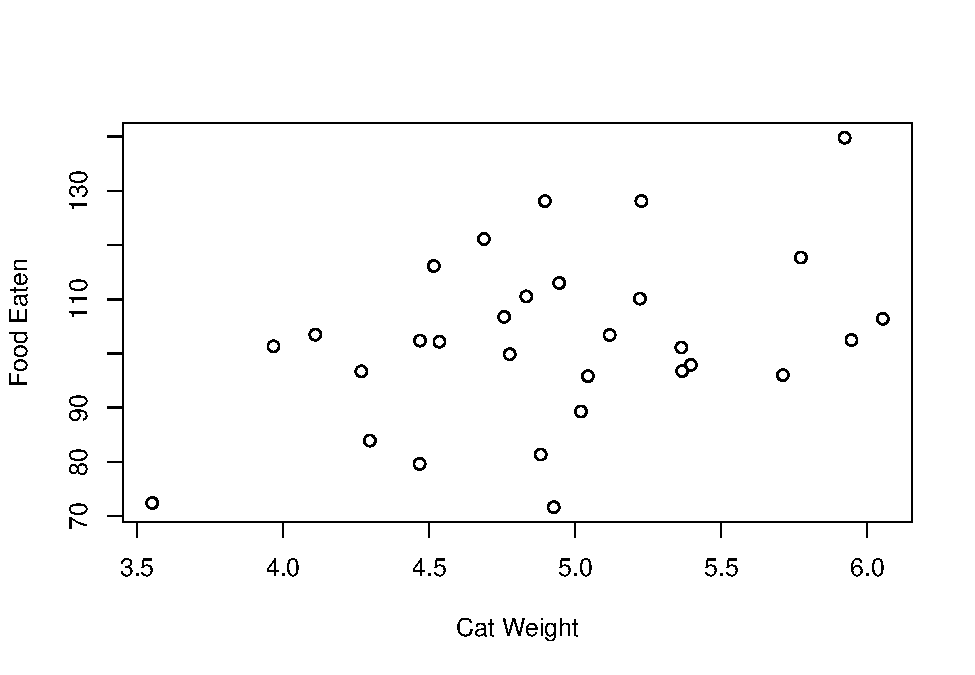
\includegraphics{Class_1_files/figure-beamer/unnamed-chunk-3-1.pdf}

\end{frame}

\begin{frame}{Four dice}

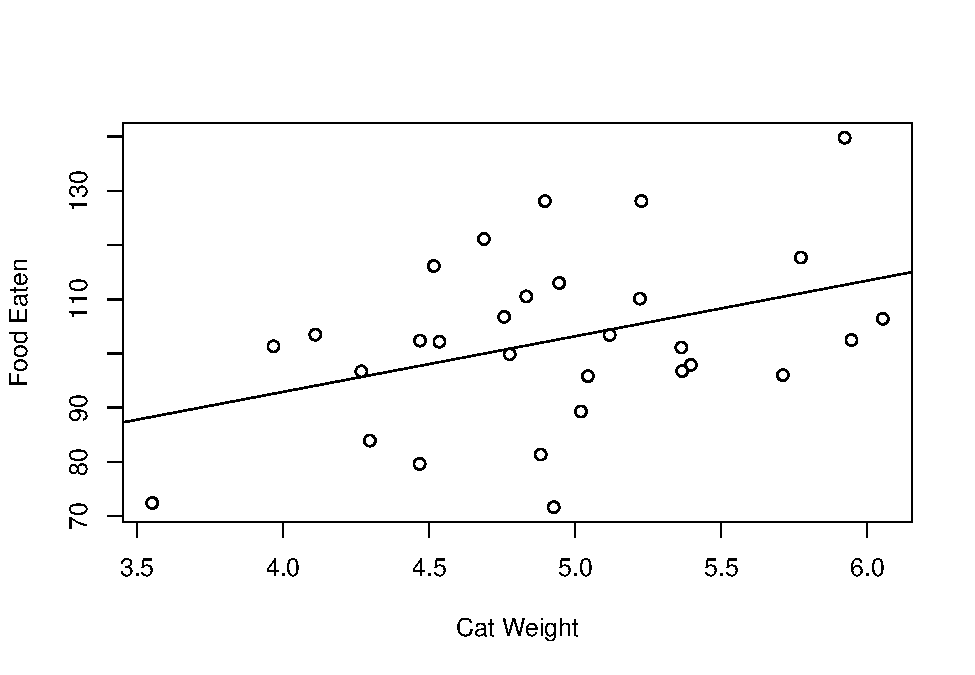
\includegraphics{Class_1_files/figure-beamer/unnamed-chunk-4-1.pdf}

\end{frame}

\begin{frame}{Ten dice}

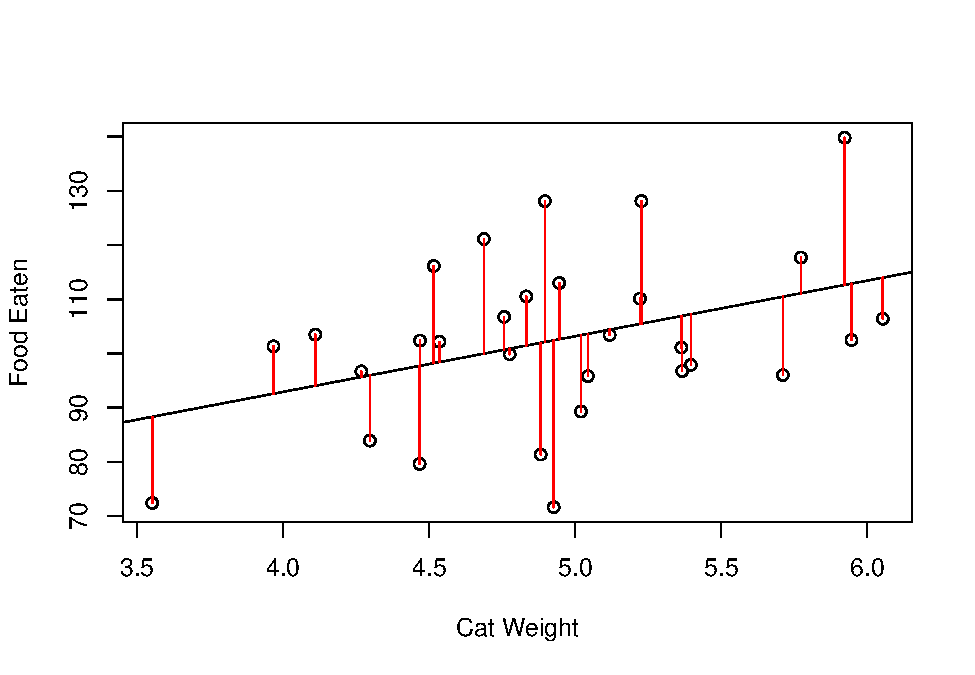
\includegraphics{Class_1_files/figure-beamer/unnamed-chunk-5-1.pdf}

\end{frame}

\begin{frame}{100 dice}

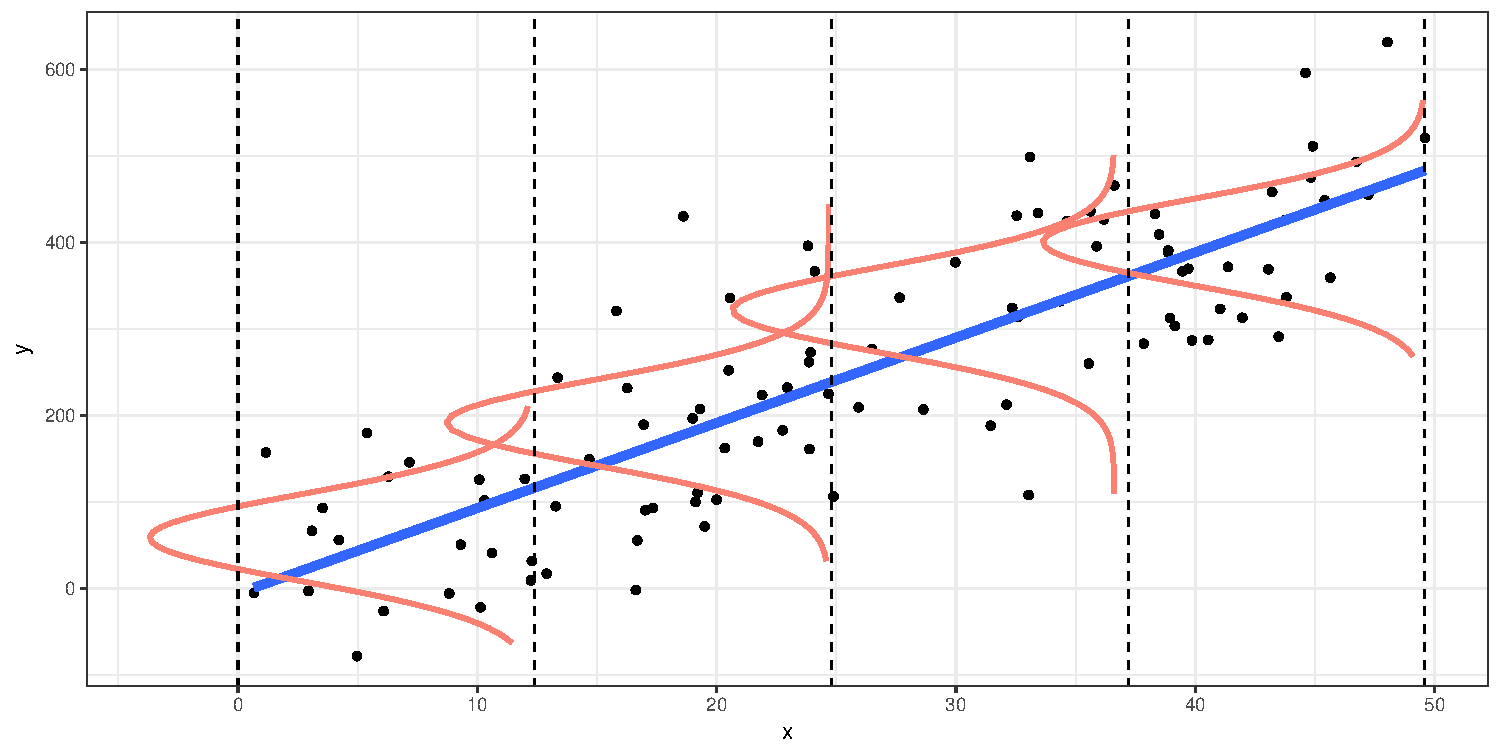
\includegraphics{Class_1_files/figure-beamer/unnamed-chunk-6-1.pdf}

\end{frame}

\begin{frame}{Do you see a pattern?}

\begin{itemize}
\itemsep1pt\parskip0pt\parsep0pt
\item
  Central limit theorem (CLT)
\end{itemize}

\begin{quote}
When sampling from a population that has a mean, provided the sample
size is large enough, the sampling distribution of the sample mean will
be close to normal regardless of the shape of the population
distribution
\end{quote}

\begin{itemize}
\itemsep1pt\parskip0pt\parsep0pt
\item
  (Technically, we were sampling the sum of X rather than the mean, but
  the mean of X is simply the sum divided by the number of observations.
  Do you care about this distintion? Didn't think so. It makes me feel
  better, though.)
\end{itemize}

\end{frame}

\begin{frame}{What does this mean?}

\begin{itemize}
\itemsep1pt\parskip0pt\parsep0pt
\item
  For our dice problem, it means that we can compute the means of our
  samples (e.g.~the mean of the 5, or 10, or 100 samples)
\item
  Remember, the \emph{sample mean} is a random variable as well, since
  it is different every time we take a sample
\item
  We can then use a \emph{continuous} probability distribution -- the
  \textbf{normal distribution} as the theoretical probability
  distribution for our random variable (i.e.~the sample mean).
\item
  This makes our life easy, because the normal distribution is very
  simple to handle mathematically (really!).
\end{itemize}

\end{frame}

\begin{frame}{Continuous probability distributions}

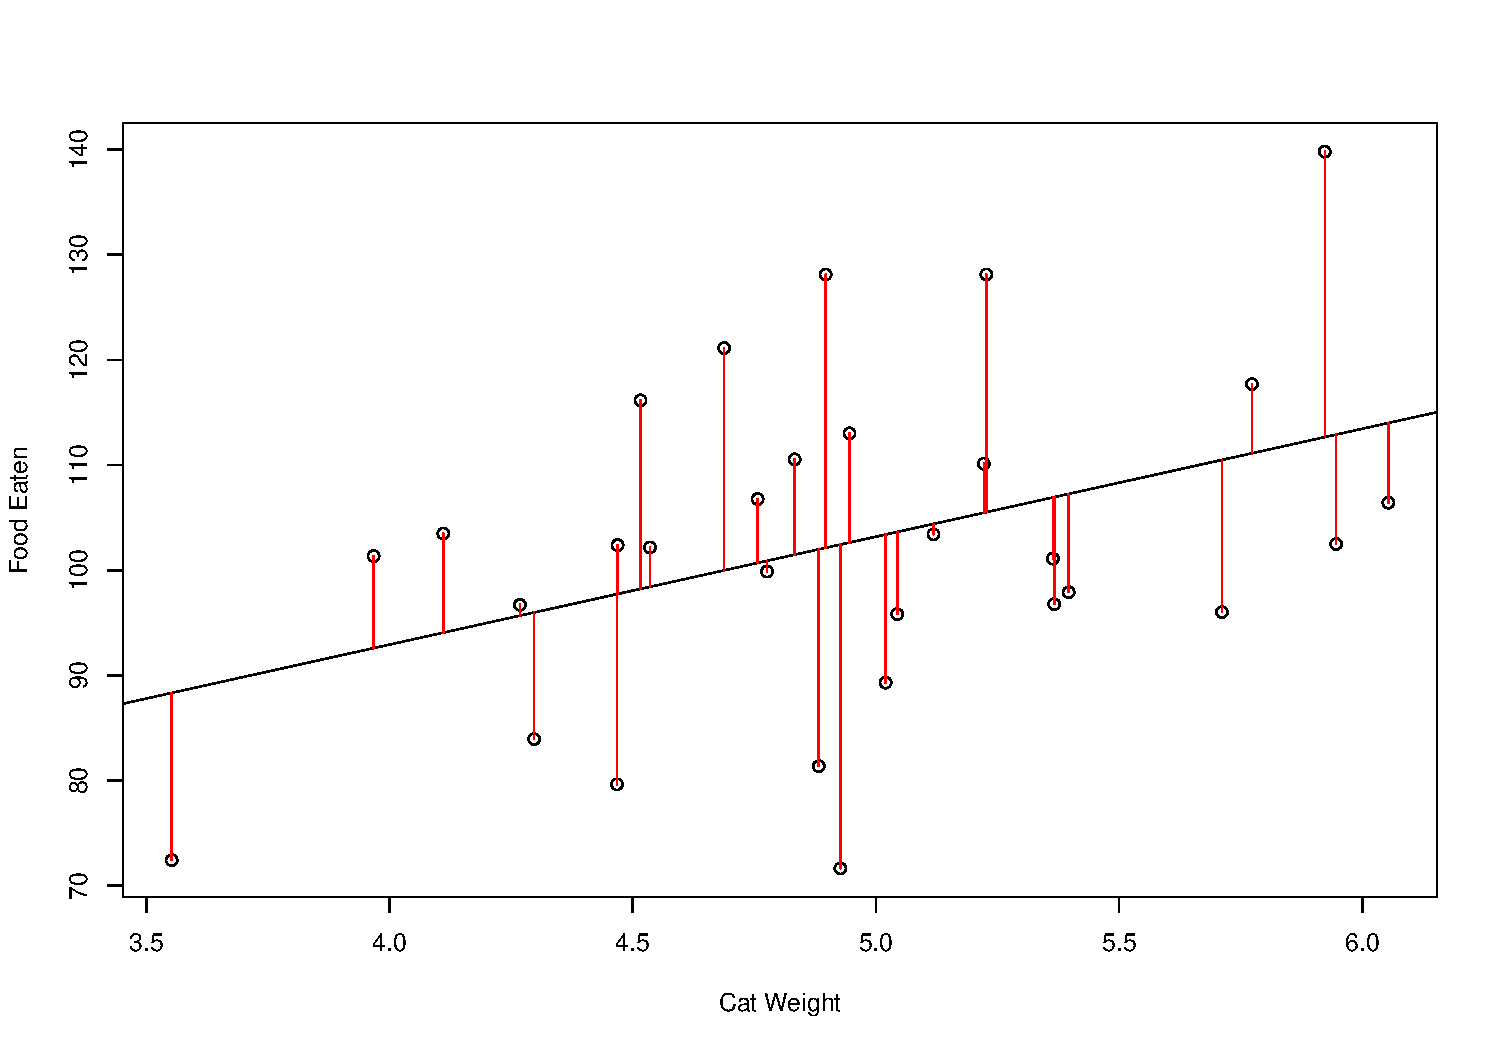
\includegraphics{Class_1_files/figure-beamer/unnamed-chunk-7-1.pdf}

Here, the outcomes are continuous, so it doesn't make sense to ask about
the probability of any point on the x-axis. - What is the probability of
x = 1? - What do you mean by ``1''? The function is continuous, so does
1.00001 still qualify as 1? - It makes more sense to ask these questions
about intervals. The probability is then the area under the curve for
the interval. - Important: the total area under the curve is 1.

\end{frame}

\begin{frame}{Normal probability density function (PDF)}

\[
  f(x,\mu,\sigma) = \frac{1}{\sigma \sqrt{2 \pi}} e^{-((x - \mu)^2/2 \sigma^2)}
\]

\includegraphics{Class_1_files/figure-beamer/unnamed-chunk-8-1.pdf}

\end{frame}

\begin{frame}{Normal probability density function (PDF)}

\[
  f(x,\mu,\sigma) = \frac{1}{\sigma \sqrt{2 \pi}} e^{-((x - \mu)^2/2 \sigma^2)}
\] - This looks scary, but it really isn't. This is simply a
mathematical function that happens to describe the distribution of a lot
of random variables in nature. - If you look closely, you can see that
the function has three parameters, \(x, \mu,\) and \(\sigma\) (\(\pi\)
and \(e\) are constants). - The first parameter, \(x\) is the random
variable. The function gives you the probability density at each value
of \(x\) - The second parameter, \(\mu\), is called the \textbf{expected
value} or the \textbf{mean} of the distribution. - The third parameter,
\(\sigma\), is called the standard deviation.

\end{frame}

\begin{frame}{Standard normal distribution}

\begin{itemize}
\itemsep1pt\parskip0pt\parsep0pt
\item
  There is an infinite number of normal distributions with different
  parameters \(\mu\) and \(\sigma\). The one with \(\mu = 0\) and
  \(\sigma = 1\) is particularly useful and is called the
  \emph{standard} normal distribution.
\item
  Look at how simple and nice the normal distribution appears when we
  plug in those values: \[
    f(z,\mu,\sigma) = \frac{1}{\sqrt{2 \pi}} e^{-z^2/2}
  \]
\item
  You can \emph{transform} values from any normal distribution to the
  normal distribution.
\item
  This is known as a \emph{z-transformation}:
  \(z = \frac{x - \mu}{\sigma}\)
\item
  By transforming all our observations to z-values and then looking up
  their probability in the standard normal distribution, this is the
  only distribution we'll ever need (\ldots{}mostly).
\end{itemize}

\end{frame}

\begin{frame}{The probability of outcomes in the standard normal
distribution}

\begin{itemize}
\itemsep1pt\parskip0pt\parsep0pt
\item
  Remember, we can't really get the probability of a \emph{point} event
  in a continuous distribution, since there are no ``points'' in a
  continuous variable
\item
  But we can ask questions about \emph{intervals}:
\item
  What's the probability of x being between 0 and 1?
\end{itemize}

\includegraphics{Class_1_files/figure-beamer/unnamed-chunk-9-1.pdf}

\end{frame}

\begin{frame}{Getting the area under the curve}

\begin{itemize}
\itemsep1pt\parskip0pt\parsep0pt
\item
  Since we know exactly what the function is, we can get the area under
  the curve.
\item
  Remember how to do that from maths class? Your best friend,
  integration :
  \[ p (0 < z < 1) = \int\limits_{0}^{1} \frac{1}{\sqrt{2 \pi}} e^{-z^2/2} dz\]
\item
  Don't want to do integration? Well, you're in luck, because most
  statistical software (and Excel!) can do this for you.
\item
  \texttt{=NORM.S.DIST(0,TRUE)} will give you the area under the curve
  to the left of 0 (i.e.~the probability that \(z < 0\))
\item
  \texttt{=NORM.S.DIST(1,TRUE)} will give you the area under the curve
  to the left of 1 (i.e.~the probability that \(z < 1\))
\end{itemize}

\end{frame}

\begin{frame}{Getting the area under the curve}

\begin{itemize}
\itemsep1pt\parskip0pt\parsep0pt
\item
  So, for our interval: \(p (0 < z < 1) = p(z < 1) - p(z < 0)\)
\item
  Remember, Excel gives us the upper tail (the area under the curve to
  the right of the \(z\) value)
\item
  So we rewrite our interval: since \(p(z < 1) = 1-p(z > 1)\) and
  \(p(z < 0) = 1-p(z > 0)\),
  \(p (0 < z < 1) = 1-p(z > 1) - (1-p(z > 0))\)
\item
  In Excel:

  \begin{itemize}
  \itemsep1pt\parskip0pt\parsep0pt
  \item
    \texttt{=NORM.S.DIST(1,TRUE)-NORM.S.DIST(0, TRUE)}
  \item
    Result: 0.3413447
  \end{itemize}
\item
  Success!
\end{itemize}

\end{frame}

\begin{frame}{Things you can do with this knowledge}

\begin{itemize}
\itemsep1pt\parskip0pt\parsep0pt
\item
  Say I'm looking at random numbers from a standard normal distribution,
  and I see that one of them is 4.
\item
  That seems very unusual
\item
  Just how unusual?

  \begin{itemize}
  \itemsep1pt\parskip0pt\parsep0pt
  \item
    What's the probability of getting a value of 4 when sampling from a
    standard normal distribution (mean = 0, sd = 1)?
  \end{itemize}
\end{itemize}

\end{frame}

\begin{frame}{Just how unusual is a value of 4?}

\begin{itemize}
\itemsep1pt\parskip0pt\parsep0pt
\item
  Remember, when you have a continuous distribution, you can't think
  about point values (e.g.~5). Rather, what you want to know is:

  \begin{itemize}
  \itemsep1pt\parskip0pt\parsep0pt
  \item
    What is the probability of getting a value of 4 \emph{or greater}
    (or \(p(z > 4) = 1-p(z < 4)\))?
  \end{itemize}
\item
  Let's ask Excel: \texttt{=1-NORM.S.DIST(4,TRUE)}

  \begin{itemize}
  \itemsep1pt\parskip0pt\parsep0pt
  \item
    Result: 0.0001338302
  \end{itemize}
\item
  So it's very unusual.
\item
  Can we come up with a similar test for our dice sample mean?
\item
  We'll have to figure out how the dice sample means are distributed.

  \begin{itemize}
  \itemsep1pt\parskip0pt\parsep0pt
  \item
    Then we can take our sample mean and see how likely (or unlikely) it
    is that it comes from the theoretical distribution.
  \end{itemize}
\end{itemize}

\end{frame}

\begin{frame}{The theoretical distribution of dice sample means}

\begin{itemize}
\itemsep1pt\parskip0pt\parsep0pt
\item
  We've seen that we can approximate our theoretical distribution (which
  is actually discrete) using a continuous distribution function, namely
  the normal distribution, which makes our lives very easy (yes,
  really!).
\item
  We have to figure out the \(\mu\) and the \(sigma\) parameters for our
  theoretical normal distribution of sample means, though.
\item
  Note for those of you who care (probably no one): In the case that we
  actually know exactly what the probabilities for our discrete
  probability distribution should look like, we could also use a
  different distribution, the \(\chi^2\) (chi square) distibution. More
  about that next week, otherwise our heads may explode.
\end{itemize}

\end{frame}

\begin{frame}{Random variables: Expected value}

\begin{itemize}
\itemsep1pt\parskip0pt\parsep0pt
\item
  Random variables have expected values
\item
  For discrete random variables, the expected value is the outcome value
  multiplied by the probability of the outcome:
  \[ E(X) = \mu = \sum\limits_{i=1}^k p(x_i)\cdot x_i\]
\item
  where \(E(X)\) is the expected value of a discrete random variable
  \(X\) with the outcomes \((x_1 \dots x_k)\) and the associated
  probabilities \((p(x_1)\dots p(x_k))\)
\item
  The equivalent for continuous random variables:
  \[\mu = \int\limits_{-\infty}^{\infty}x f(x) dx\]
\end{itemize}

\end{frame}

\begin{frame}{Random variables: Variance}

\begin{itemize}
\itemsep1pt\parskip0pt\parsep0pt
\item
  Random variables also have variances
\item
  For discrete random variables, the variance is the difference between
  the outcome value and the mean multiplied by the probability of the
  outcome: \[ \sigma^2 = \sum\limits_{i=1}^k p(x_i)\cdot (x_i - \mu)^2\]
\item
  where \(\sigma^2\) is the variance of a discrete random variable \(X\)
  with the outcomes \((x_1 \dots x_k)\) and the associated probabilities
  \((p(x_1)\dots p(x_k))\)
\item
  The equivalent for continuous random variables:
  \[\mu = \int\limits_{-\infty}^{\infty}(x-\mu)^2 f(x) dx\]
\end{itemize}

\end{frame}

\begin{frame}{Maths basics: Expected values}

\begin{itemize}
\itemsep1pt\parskip0pt\parsep0pt
\item
  For example, the expected value \(\mu\) of rolling a six-sided die is:
  \[
  \begin{aligned}
  E(X) &= \sum\limits_{i=1}^{6} p(x_i) \cdot x_i \\
  &= x_1 \cdot p(x_1) + x_2 \cdot p(x_2) + x_3 \cdot p(x_3) + x_4 \cdot p(x_4) \\ 
  &+ x_5 \cdot p(x_5) + x_6 \cdot p(x_6) \\
  &= 1 \cdot \frac{1}{6} + 2 \cdot \frac{1}{6} + 3 \cdot \frac{1}{6} + 4 \cdot \frac{1}{6} \\ 
  &+ 5 \cdot \frac{1}{6} + 6 \cdot \frac{1}{6} \\
  &= \frac{21}{6} = 3.5
  \end{aligned}
  \]
\end{itemize}

\end{frame}

\begin{frame}{Maths basics: Variance}

\begin{itemize}
\itemsep1pt\parskip0pt\parsep0pt
\item
  For example, the variance \(\sigma^2\) of rolling a six-sided die is:
  \[
  \begin{aligned}
  \sigma^2 &= \sum\limits_{i=1}^6 p(x_i)\cdot (x_i - \mu)^2 \\
  &= (x_1-\mu)^2 \cdot p(x_1) + (x_2-\mu)^2 \cdot p(x_2) + (x_3-\mu)^2 \cdot p(x_3) \\
  &+ (x_4-\mu)^2 \cdot p(x_4) + (x_5-\mu)^2 \cdot p(x_5) + (x_6-\mu)^2 \cdot p(x_6) \\
  &= \frac{1}{6}\cdot \Big((1-3.5)^2 + (2-3.5)^2 + (3-3.5)^2 \\
  &+ (4-3.5)^2 + (5-3.5)^2+ (6-3.5)^2\Big) \\
  &= \frac{17.5}{6} = 2.9167
  \end{aligned}
  \]
\end{itemize}

\end{frame}

\begin{frame}{Back to the dice example again}

\begin{itemize}
\itemsep1pt\parskip0pt\parsep0pt
\item
  So, we know that, if our dice are fair, our dice rolls come from a
  discrete theoretical distribution with \(\mu = 3.5\) and
  \(\sigma^2 = 2.9167\).
\item
  But remember, we don't want to evaluate single dice rolls, but rather
  the mean of a sample of dice rolls, since that will enable us to use
  the nice and easy normal distribution to calculate the probabilities.
\item
  So, what is the mean \(\mu_{\bar{x}}\) and what is the variance
  \(\sigma_{\bar{x}^2}\) for the \textbf{distribution of sample means}?
\end{itemize}

\end{frame}

\begin{frame}{Maths basics: Expected values (3)}

\begin{itemize}
\itemsep1pt\parskip0pt\parsep0pt
\item
  What is the expected value of rolling two dice and adding the spots?
\item
  What is the expected value of rolling two dice and multiplying the
  number of spots?
\item
  What is the expected value of an IQ test result?
\item
  Imagine you and your friend both take IQ tests. What is the expected
  value of the differences between your scores (assuming that you both
  come from the general population)?

  \begin{itemize}
  \itemsep1pt\parskip0pt\parsep0pt
  \item
    Don't know? Well, stay tuned. This will require some maths, though.
  \end{itemize}
\end{itemize}

\end{frame}

\begin{frame}{Maths basics: Computing expected values}

\begin{itemize}
\itemsep1pt\parskip0pt\parsep0pt
\item
  The expected value of a random variable is often also called \(\mu\):
  \[E(X) = \mu\]
\item
  \(\mu\) is also called the distribution \emph{mean}
\item
  What if the expected value is constant across all the possible
  outcomes?
\item
  e.g what is the expected value of a die with 1 on all sides?

  \begin{itemize}
  \itemsep1pt\parskip0pt\parsep0pt
  \item
    1, of course!
  \end{itemize}
\item
  More general:
\item
  if the value is the same across all outcomes, we can call it a
  constant
\item
  e.g.~if \(x_1 = x_2 = x_3 = \dots = x_i = 1\)

  \begin{itemize}
  \itemsep1pt\parskip0pt\parsep0pt
  \item
    then \(E(X) = E(1) = 1\)
  \end{itemize}
\end{itemize}

\end{frame}

\begin{frame}{Maths basics: Computing expected values (2)}

Even more general: If a is a constant, then \(E(a) = a\) - If \(X\) is a
random variable and \(a\) is a constant, what is the expected value of
\(a \cdot X\)? \[E(a\cdot X) = a \cdot E(X)\] - For example, if the
expected value of rolling a 6-sided die is 3.5, what is the expected
value of rolling a 6-sided die and then multiplying the number of spots
by 3? \[ E(3\cdot X) = 3\cdot E(X) = 3\cdot 3.5 = 10.5\] - Try it if you
don't believe me!

\end{frame}

\begin{frame}{Maths basics: Computing expected values (3)}

\begin{itemize}
\itemsep1pt\parskip0pt\parsep0pt
\item
  If \(X\) is a random variable and \(a\) is a constant, what is the
  expected value of \(a + X\)? \[E(a + X) = a + E(X)\]
\item
  For example, if the expected value of rolling a 6-sided die is 3.5,
  what is the expected value of rolling a 6-sided die and then adding 3
  to the number of spots? \[ E(3 + X) = 3 + E(X) = 3 + 3.5 = 6.5\]
\item
  Try it if you still don't believe me!
\end{itemize}

\end{frame}

\begin{frame}{Maths basics: Computing expected values (4)}

\begin{itemize}
\itemsep1pt\parskip0pt\parsep0pt
\item
  If \(X\) is a random variable and \(Y\) is a random variable, what is
  the expected value of \(X + Y\)? \[E(X + Y) = E(X) + E(Y)\]
\item
  For example, if the expected value of rolling two 6-sided dice and
  adding the two results? \[ E(X + Y) = E(X) + E(Y)= 3.5 + 3.5 = 7\]
\item
  Try it if you still don't believe me!
\end{itemize}

\end{frame}

\begin{frame}{Maths basics: Computing expected values (5)}

\begin{itemize}
\itemsep1pt\parskip0pt\parsep0pt
\item
  If \(X\) is a random variable and \(Y\) is a random variable, what is
  the expected value of \(X \cdot Y\)?
  \[E(X \cdot Y) = E(X) \cdot E(Y)\]
\item
  But \emph{ONLY} if \(X\) and \(Y\) are \emph{INDEPENDENT}
\item
  For example, if the expected value of rolling two 6-sided dice and
  multiplying the two results?
  \[ E(X + Y) = E(X) \cdot E(Y)= 3.5 \cdot 3.5 = 12.25\]
\item
  Try it if you still don't believe me!
\end{itemize}

\end{frame}

\begin{frame}{The expected value of the sample mean}

\begin{itemize}
\itemsep1pt\parskip0pt\parsep0pt
\item
  If \(X\) is a random variable, and we take a sample of size \(n\) from
  \(X\), what is the expected value of the mean of that sample?
\item
  Remember, this is how you compute the sample mean:
  \[\bar{x} = \frac{\sum\limits_{i=1}^{n}}{n}\]
\item
  The expected value of the sample mean is: \[
  \begin{aligned}
  E(\bar{X}) &= E\Bigg(\frac{\sum\limits_{i=1}^{n}}{n}\Bigg)\\
         &= \frac{1}{n}\cdot\big(E\sum\limits_{i=1}^n{X_i}\big)
  \end{aligned}\]
\end{itemize}

\end{frame}

\begin{frame}{The expected value of the sample mean (2)}

\[
\begin{aligned}
           &= \frac{1}{n}\cdot\big(E\sum\limits_{i=1}^n{X_i}\big) \text{ (since } E(a\cdot X) = a \cdot E(X)\text{)} \\
           &= \frac{1}{n}\cdot\sum\limits_{i=1}^n{E(X_i)} \text{ (since } E(X+Y) = E(X) + E(Y)\text{)} \\
           &= \frac{1}{n}\cdot\sum\limits_{i=1}^n{\mu_x} \text{ (since } E(X) = \mu \text{)} \\
           &= \frac{1}{n}\cdot n \cdot\mu_x = \mu_x
\end{aligned}\]

\end{frame}

\begin{frame}{The expected value of the sample mean (3)}

\begin{itemize}
\itemsep1pt\parskip0pt\parsep0pt
\item
  We just found that the expected value of the sample mean
  \(E(\bar{X})\) is identical to the expected value (the mean) of the
  population \(\mu_x\), \emph{regardless of the sample size}.
\item
  We can say that the sample mean \(\overline{X}\) is an \emph{unbiased
  estimator} of the population mean \(\mu\)
\item
  No matter what we do and what crazy population we're taking samples
  of, the sample means will always be distributed around the true
  population mean.

  \begin{itemize}
  \itemsep1pt\parskip0pt\parsep0pt
  \item
    \emph{Isn't that cool?}
  \item
    I know what you're thinking right now, but this is \emph{actually}
    cool. Just think about it: If you want to know the true population
    mean of any population, all you have to do is take enough samples.
  \end{itemize}
\end{itemize}

\end{frame}

\begin{frame}{Our dice example}

\begin{itemize}
\itemsep1pt\parskip0pt\parsep0pt
\item
  Remember, we want to know how the means of our dice rolls should be
  distributed if the dice are fair. So, now we know that they are
  normally distributed (because of the Central Limit Theorem) with an
  expected value of \(\mu_{\bar{x}} = 3.5\).
\item
  What about the \emph{variance} of the \emph{distribution of sample
  means}?

  \begin{itemize}
  \itemsep1pt\parskip0pt\parsep0pt
  \item
    Well, this will take some work. Sorry, people. It's maths time.
  \item
    First, we need to know how the sample variance is related to the
    population variance.
  \item
    In other words, we need to know the expected value of the sample
    variance.
  \end{itemize}
\end{itemize}

\end{frame}

\begin{frame}{The expected value of the sample variance}

\begin{itemize}
\itemsep1pt\parskip0pt\parsep0pt
\item
  OK, first we want to know how the variance of your samples (\(s^2\))
  is related to the population variance \(\sigma^2\).
\item
  Remember that the variance of a sample is
  \[ s^2 = \frac{\sum\limits_{i=1}^{n}(x_i - \bar{x})^2}{n}\]
\item
  We can rewrite this as: \[
  \begin{aligned}
  s^2 &= \frac{\sum\limits_{i=1}^{n}(x_i - \bar{x})^2}{n} = \frac{\sum\limits_{i=1}^{n}(x_i^2 - 2\cdot x_i + \bar{x})^{2}}{n}\\
  &=\frac{\sum\limits_{i=1}^{n}x_i^2 - 2\cdot \bar{x} \cdot\sum\limits_{i=1}^{n}x_i + \bar{x}^{2}}{n}
  \end{aligned}
  \]
\end{itemize}

\end{frame}

\begin{frame}{The expected value of the sample variance (2)}

\begin{itemize}
\itemsep1pt\parskip0pt\parsep0pt
\item
  Further rewriting: Since
  \(\sum\limits_{i=1}^{n} x_i = n \cdot \bar{x}\) : \[
  \begin{aligned}
  s^2 &=\frac{\sum\limits_{i=1}^{n}x_i^2 - 2\cdot \bar{x} \cdot\sum\limits_{i=1}^{n}x_i + \bar{x}^{2}}{n}\\
  &= \frac{\sum\limits_{i=1}^{n}x_i^2 - 2\cdot \bar{x} \cdot n \cdot \bar{x} + \bar{x}^{2}}{n}\\
  &= \frac{\sum\limits_{i=1}^{n}x_i^2 - n\cdot \bar{x}^2}{n} = \frac{\sum\limits_{i=1}^{n}x_i^2}{n} - \bar{x}^2
  \end{aligned}
  \]
\end{itemize}

\end{frame}

\begin{frame}{The expected value of the sample variance (3)}

\begin{itemize}
\itemsep1pt\parskip0pt\parsep0pt
\item
  Now we can calculate the expected value of \(s^2\): \[
  \begin{aligned}
  E(S^2) &= E\Bigg(\frac{\sum\limits_{i=1}^{n}X_i^2}{n} - \bar{X}^2\Bigg) \\
     &= E\Bigg(\frac{\sum\limits_{i=1}^{n}X_i^2}{n}\Bigg) - E(\bar{X}^2) \\
     &= \frac{\sum\limits_{i=1}^{n}E(X_i^2)}{n} - E(\bar{X}^2) = \frac{n\cdot E(X_i^2)}{n}-E(\bar{X}^2)
  \end{aligned}
  \]
\end{itemize}

\end{frame}

\begin{frame}{The expected value of the sample variance (4)}

\begin{itemize}
\itemsep1pt\parskip0pt\parsep0pt
\item
  And \(\frac{n\cdot E(X_i^2)}{n}-E(\bar{X}^2)\) of course simplifies to
  \(E(X_i^2)-E(\bar{X}^2)\)
\item
  So, now we have to figure out what \(E(X_i^2)\) and \(E(\bar{X}^2)\)
  are.
\item
  The ``easiest'' (I know, right?) way to do this is to start with the
  population variance \(\sigma^2\) and the variance of the sample means
  \(\sigma_{\bar{x}}^2\)
\end{itemize}

\end{frame}

\begin{frame}{The expected value of the sample variance (5)}

\begin{itemize}
\itemsep1pt\parskip0pt\parsep0pt
\item
  We can define the population variance as
  \(\sigma^2 = E(X_i - \mu)^2\), the expected value of the squared
  deviations of \(X\) from the population mean \(\mu\)
\item
  Let's rewrite this: \[
  \begin{aligned}
  \sigma^2 &= E(X_i - \mu)^2 = E(X_i^2 - 2X_i\mu + \mu^2) \\
       &= E(X_i^2) - E(2X_i\mu) + E(\mu^2)\\
       &= E(X_i^2) - 2\mu E(X_i) + \mu^2
  \end{aligned}
  \] since \(\mu\) is a constant (and \(\mu^2\) is too, of course).
\end{itemize}

\end{frame}

\begin{frame}{The expected value of the sample variance (6)}

Continuing from previous slide: - We already determined that
\(\mu = E(X)\), so: \[
\begin{aligned}
\sigma^2 &= E(X_i^2) - 2\mu E(X_i) + \mu^2 \\
         &= E(X_i^2) - 2\mu^2 + \mu^2 = E(X_i^2) - \mu^2 
\end{aligned}
\] - Solving for \(E(X_i^2)\): \[\begin{aligned}
\sigma^2 &= E(X_i^2) - \mu^2  \\
&\Leftrightarrow E(X_i^2) = \sigma^2 + \mu^2
\end{aligned}
\] - OK, so now we know that the expected value of a squared random
variable is equal to the sum of the population variance \(\sigma^2\) and
the square of the population mean \(\mu^2\).

\end{frame}

\begin{frame}{The expected value of the sample variance (7)}

\begin{itemize}
\itemsep1pt\parskip0pt\parsep0pt
\item
  Next up: the variance of sample means \(\sigma_{\bar{x}}^2\)

  \begin{itemize}
  \itemsep1pt\parskip0pt\parsep0pt
  \item
    This is the square of the \emph{standard error} of the mean
    \(\sigma_{\bar{x}}\)
  \end{itemize}
\item
  We can define the variance of sample means as
  \(\sigma_{\bar{x}}^2 = E(\bar{X} - \mu)^2\), i.e.~the expected value
  of the squared deviations of the sample means from the true population
  mean
\item
  We can rewrite this just like we did for the sample variance (this
  works exactly the same as before; if you are bored, you can skip the
  next two slides).
\end{itemize}

\end{frame}

\begin{frame}{The expected value of the sample variance (7a)}

\begin{itemize}
\itemsep1pt\parskip0pt\parsep0pt
\item
  We can define the variance of the sample means as
  \(\sigma_{\bar{x}}^2 = E(\bar{X} - \mu)^2\)
\item
  Let's rewrite this: \[
  \begin{aligned}
  \sigma^2 &= E(\bar{X} - \mu)^2 = E(\bar{X}^2 - 2\bar{X}\mu + \mu^2) \\
       &= E(\bar{X}^2) - E(2\bar{X}\mu) + E(\mu^2)\\
       &= E(\bar{X}^2) - 2\mu E(\bar{X}) + \mu^2
  \end{aligned}
  \] since \(\mu\) is a constant (and \(\mu^2\) is too, of course).
\end{itemize}

\end{frame}

\begin{frame}{The expected value of the sample variance (7b)}

Continuing from previous slide: - We already determined that
\(\mu = E(\bar{X})\), so: \[
\begin{aligned}
\sigma_{\bar{x}}^2 &= E(\bar{X}^2) - 2\mu E(\bar{X}) + \mu^2 \\
         &= E(\bar{X}^2) - 2\mu^2 + \mu^2 = E(\bar{X}^2) - \mu^2 
\end{aligned}
\] - Solving for \(E(\bar{X}^2)\): \[\begin{aligned}
\sigma_{\bar{x}}^2 &= E(\bar{X}^2) - \mu^2  \\
&\Leftrightarrow E(\bar{X}^2) = \sigma_{\bar{x}}^2 + \mu^2
\end{aligned}
\] - OK, so now we know that the expected value of the squared mean of a
random variable is equal to the sum of the variance of the sample means
\(\sigma_{\bar{x}}^2\) and the square of the population mean \(\mu^2\).

\end{frame}

\begin{frame}{The expected value of the sample variance (8)}

\begin{itemize}
\itemsep1pt\parskip0pt\parsep0pt
\item
  Plugging \(E(X_i^2) = \sigma^2 + \mu^2\) and
  \(E(\bar{X}^2) = \sigma_{\bar{x}}^2 + \mu^2\) into our term for the
  expected value of the sample variance: \[
  \begin{aligned}
  E(S^2) &= E(X_i^2)-E(\bar{X}^2) = \sigma^2 + \mu^2 - (\sigma_{\bar{x}}^2 + \mu^2) \\
     &= \sigma^2 - \sigma_{\bar{x}}^2
  \end{aligned}
  \]
\item
  In words: the expected value of the sample variance is equal to the
  population variance minus the variance of the sample means.

  \begin{itemize}
  \itemsep1pt\parskip0pt\parsep0pt
  \item
    This means that the sample variance \emph{systematically}
    underestimates the population variance
  \item
    The sample variance is \emph{NOT} an unbiased estimator of the
    population variance.
  \end{itemize}
\end{itemize}

\end{frame}

\begin{frame}{The expected value of the variance of sample means}

\begin{itemize}
\itemsep1pt\parskip0pt\parsep0pt
\item
  We start with the relationship we just figured out:
  \(E(\sigma_{\bar{x}}^2) = \sigma_{\bar{x}}^2 = E(\bar{X}^2)-\mu^2\)
  (since \(E(\bar{X}^2)\) and \(\mu^2\) are both constants).
\item
  We can rewrite \(\bar{X}^2\) as: \[
  \begin{aligned} 
  \bar{X}^2 &= \frac{(X_1+X_2+\dots+X_n)^2}{n^2} \\
        &= \frac{1}{n^2}\cdot \Bigg(X_1^2+X_2^2 + \dots+X_n^2 \\
        &+2\sum\limits_{i=1}{\sum\limits_{j=i+1}{X_i\cdot X_j}}\Bigg)
  \end{aligned}
  \]
\end{itemize}

\end{frame}

\begin{frame}{The expected value of the variance of sample means (2)}

\begin{itemize}
\itemsep1pt\parskip0pt\parsep0pt
\item
  If (and only if!) \(X_1, X_2,\dots, X_n\) are independent (i.e.~the
  value of \(X_1\) doesn't depend on the value of \(X_2\), or \(X_3\),
  etc.), we can write the expected value of the final term of this
  expression as: \[
  \begin{aligned}
  E\Bigg(2\sum\limits_{i=1}^{n-1}{\sum\limits_{j=i+1}^{n}{X_i\cdot X_j}}\Bigg) &= n\cdot*(n-1)\cdot E(X_i)\cdot E(X_j)\\
  &= n\cdot(n-1)\cdot\mu^2
  \end{aligned}
  \]
\item
  Since \(E(\sum_{i=1}^{n}X_i) = \sum_{i=1}^{n}E(X_i)\) and
  \(E(X_i) = \mu\)
\end{itemize}

\end{frame}

\begin{frame}{The expected value of the variance of sample means (3)}

\begin{itemize}
\itemsep1pt\parskip0pt\parsep0pt
\item
  With that, we can rewrite \(E(\bar{X^2})\) as \[
  \begin{aligned}
  E(\bar{X^2}) &= \frac{1}{n^2}\cdot \Big(E(X_1)^2 + E(X_2)^2 + \dots \\
           &+ E(X_n)^2) + n \cdot (n-1)\cdot \mu^2\Big)
  \end{aligned}\]
\item
  But we know already (through our hard work earlier) that the expected
  value of the square of \(X_i\) is \(E(X_i^2) = \sigma^2 + \mu^2\).
\item
  So we can replace \(E(X_1)^2 + E(X_2)^2 + \dots + E(X_n)^2\) with
  \(n\cdot(\sigma^2 + \mu^2) = n\cdot \sigma^2 + n\cdot \mu^2\).
\end{itemize}

\end{frame}

\begin{frame}{The expected value of the variance of sample means (4)}

\begin{itemize}
\itemsep1pt\parskip0pt\parsep0pt
\item
  Let's do that now: \[
  \begin{aligned}
  E(\bar{X^2}) &= \frac{1}{n^2}\cdot \Big(n\cdot \sigma^2 + n\cdot \mu^2+ n \cdot (n-1)\cdot \mu^2\Big)\\
           &= \frac{\sigma^2}{n}+\frac{n\cdot \mu^2+n*2\cdot\mu^2-n\cdot\mu^2}{n^2} = \frac{\sigma^2}{n}+\mu^2
  \end{aligned}\]
\item
  Plugging this into our previous equation
  \(\sigma_{\bar{x}}^2 = E(\bar{X}^2) - \mu^2\) we get:
  \[\sigma_{\bar{x}}^2 = \frac{\sigma^2}{n}+\mu^2 - \mu^2 = \frac{\sigma^2}{n}\]
\item
  If we take the square root of this, we \emph{FINALLY} get the
  \textbf{standard error of the mean}:
  \[\sigma_{\bar{x}} = \sqrt{\frac{\sigma^2}{n}} = \frac{\sigma}{\sqrt{n}}\]
\end{itemize}

\end{frame}

\begin{frame}{Correcting the bias in the expected value of the sample
variance}

\begin{itemize}
\itemsep1pt\parskip0pt\parsep0pt
\item
  Before we actually use our hard-earned \(\mu_{\bar{x}}\) and
  \(\sigma_{\bar{x}}\), a quick detour:
\item
  Remember that the expected value of the sample variance was biased by
  the variance of the sample mean, i.e.
  \(E(S^2) = \sigma^2 - \sigma_{\bar{x}}^2\)?
\item
  Now we know what the variance of the sample mean is, so let's plug it
  in: \[
  \begin{aligned}
  E(S^2) &= \sigma^2 - \sigma_{\bar{x}}^2 = \sigma^2 - \frac{\sigma^2}{n} = \frac{n\cdot\sigma^2-\sigma^2}{n} \\
     &= \sigma^2\cdot\frac{n-1}{n}
  \end{aligned}
  \]
\end{itemize}

\end{frame}

\begin{frame}{Correcting the bias in the expected value of the sample
variance (2)}

\begin{itemize}
\itemsep1pt\parskip0pt\parsep0pt
\item
  We just found out that the expected value of the sample variance
  \(E(s^2)\) underestimates the true population variance \(\sigma^2\) by
  a factor of \(\frac{n-1}{n}\).
\item
  That means we can apply a correction factor to the sample variance so
  that it becomes an \emph{unbiased} estimator of the population
  variance: \[
  \begin{aligned}
  s_{n-1}^2 &= s^2 / \frac{n-1}{n} =  s^2\cdot\frac{n}{n-1} = \frac{\sum\limits_{i=1}^n(x_i-\bar{x})^2}{n}\cdot\frac{n}{n-1}\\
        &= \frac{\sum\limits_{i=1}^n(x_i-\bar{x})^2}{n-1}
  \end{aligned}
  \]
\end{itemize}

\end{frame}

\begin{frame}{Correcting the bias in the expected value of the sample
variance (3)}

\begin{itemize}
\itemsep1pt\parskip0pt\parsep0pt
\item
  Most statistical software will use this corrected formula for
  computing the sample variance:
  \(s_{n-1}^2 = \frac{\sum\limits_{i=1}^n(x_i-\bar{x})^2}{n-1}\)
\item
  If you want a more intuitive explanation of what is going on here,
  watch the videos at EasyStats:
  \href{http://easystats.org/}{\url{http://easystats.org/}}
\end{itemize}

\end{frame}

\begin{frame}{Please, let's FINALLY finish the dice example}

\begin{itemize}
\itemsep1pt\parskip0pt\parsep0pt
\item
  OK, OK. We now have everything we need to determine whether our dice
  roll sample mean is unusual assuming fair dice.
\item
  More formally, we call this a \textbf{Hypothesis Test}
\item
  We establish a \emph{Null Hypothesis} \(H_0\) (e.g.~the dice are
  fair),

  \begin{itemize}
  \itemsep1pt\parskip0pt\parsep0pt
  \item
    determine a theoretical probability distribution of the random
    variable (our dice roll means) given that the \(H_0\) is true:

    \begin{itemize}
    \itemsep1pt\parskip0pt\parsep0pt
    \item
      a normal distribution with \(\mu_{\bar{x}} = 3.5\) and
      \(\sigma_{\bar{x}} = \frac{\sigma}{\sqrt{n}} = \frac{\sqrt{2.9167}}{\sqrt{n}}\),
      where n is the number of dice rolls in our sample,
    \end{itemize}
  \item
    and finally we can calculate the probability that you would observe
    the sample mean you observed given the \(H_0\).
  \end{itemize}
\end{itemize}

\end{frame}

\begin{frame}{Final steps}

\begin{itemize}
\itemsep1pt\parskip0pt\parsep0pt
\item
  So, let's assume you did 10 dice rolls for this example, and that your
  mean was 4.
\item
  Since we know that the sample means should be normally distributed, we
  can transform your mean into a \emph{z}-value:
\item
  Since \(\mu_{\bar{x}} = 3.5\) and
  \(\sigma_{\bar{x}} = \frac{\sigma}{\sqrt{n}} = \frac{\sqrt{2.9167}}{\sqrt{10}} = 0.5400648\):
  \[ z(4) = \frac{4-3.5}{0.5400648}=0.9258148\]
\item
  Let's ask Excel what the probability of observing a sample mean this
  far away (or farther) from the population mean is for the standard
  normal distribution: \texttt{1-NORM.S.DIST(0.9258,TRUE)}

  \begin{itemize}
  \itemsep1pt\parskip0pt\parsep0pt
  \item
    Result: 0.177274964
  \end{itemize}
\end{itemize}

\end{frame}

\begin{frame}{Final steps (2)}

\begin{itemize}
\itemsep1pt\parskip0pt\parsep0pt
\item
  Fisher (who popularised this sort of hypothesis testing) suggested
  that we should consider data with a probability of less than 5\% (or
  .05) given the null hypothesis as \textbf{significant} evidence for
  rejecting the null hypothesis.
\item
  In our case, we are far away from a probability (or short,
  \emph{p}-value) of .05. So, we can't reject the null hypothesis. Try
  it for yourselves, though.
\item
  More on this next week.
\end{itemize}

\end{frame}

\begin{frame}{Technical note for those who really care}

\begin{itemize}
\itemsep1pt\parskip0pt\parsep0pt
\item
  We really don't care about the direction of the effect here, just the
  absolute distance from the mean (i.e.~this is a \emph{two-tailed}
  test).
\item
  So, to be absolutely correct, we should ask Excel to give us the
  probability of z being at least this far away from the mean on either
  side:
  \(p(z < -.9258 \cup z > .9258) \\= p(z < -.9258) + (1-p(z < .9258))\).
\item
  When we ask Excel for the p-value
  \texttt{=NORM.S.DIST(-0.9258,TRUE)+(1-NORM.S.DIST(0.9258,TRUE))} we
  get the actual, correct result of 0.3545499.
\item
  Good times. Until next week!
\end{itemize}

\end{frame}
